\begin{table}[]
\centering
\label{data_sources}
\caption{Origins of labeled training data}
\begin{tabular}{|r|r|l|}
\hline
Amount & Label & Origin \\ \hline
9 & DATA & Manual Google search for Open Data
repositories \\ \hline
82 & DATA & Repositories of GitHub user `datasets' \\ \hline
17 & EDU & GitHub Search for ``course, material'' \\ \hline
17 & DOCS & GitHub Search for ``documentation'' \\ \hline
423 & WEB & Google Search for ``site:.github.io'' \\ \hline
58 & HW & GitHub Search for ``homework, assignments,
solution'' \\ \hline
13 & DEV & Showcases ``Virtual Reality'' \\ \hline
12 & DEV & Showcases ``Software Development Tools'' \\ \hline
14 & DEV & Showcases ``Front-end JavaScript frameworks'' \\ \hline
20 & DEV & Showcases ``DevOps tools'' \\ \hline
16 & DEV & Showcases ``Text editors'' \\ \hline
24 & DEV & Showcases ``Game Engines'' \\ \hline
27 & DEV & Showcases ``Web Application Frameworks'' \\ \hline
42 & DEV & Showcases ``Programming Languages'' \\ \hline
180 & DOCS & GitHub Repo Content: awesome-awesomeness \\ \hline
6 & DATA & Showcases ``Open Data'' \\ \hline
86 & HW & Github Search for ``homework, solution'' \\ \hline
\end{tabular}
\end{table}

\begin{figure}[H]
	\centering
		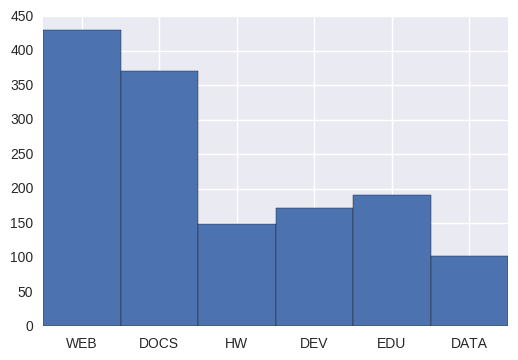
\includegraphics[width=10cm]{graphics/training_data_distribution.png}
	\caption{Training Data Distribution}
	\label{training_data_distribution}
\end{figure}


\begin{figure}
	\centering
		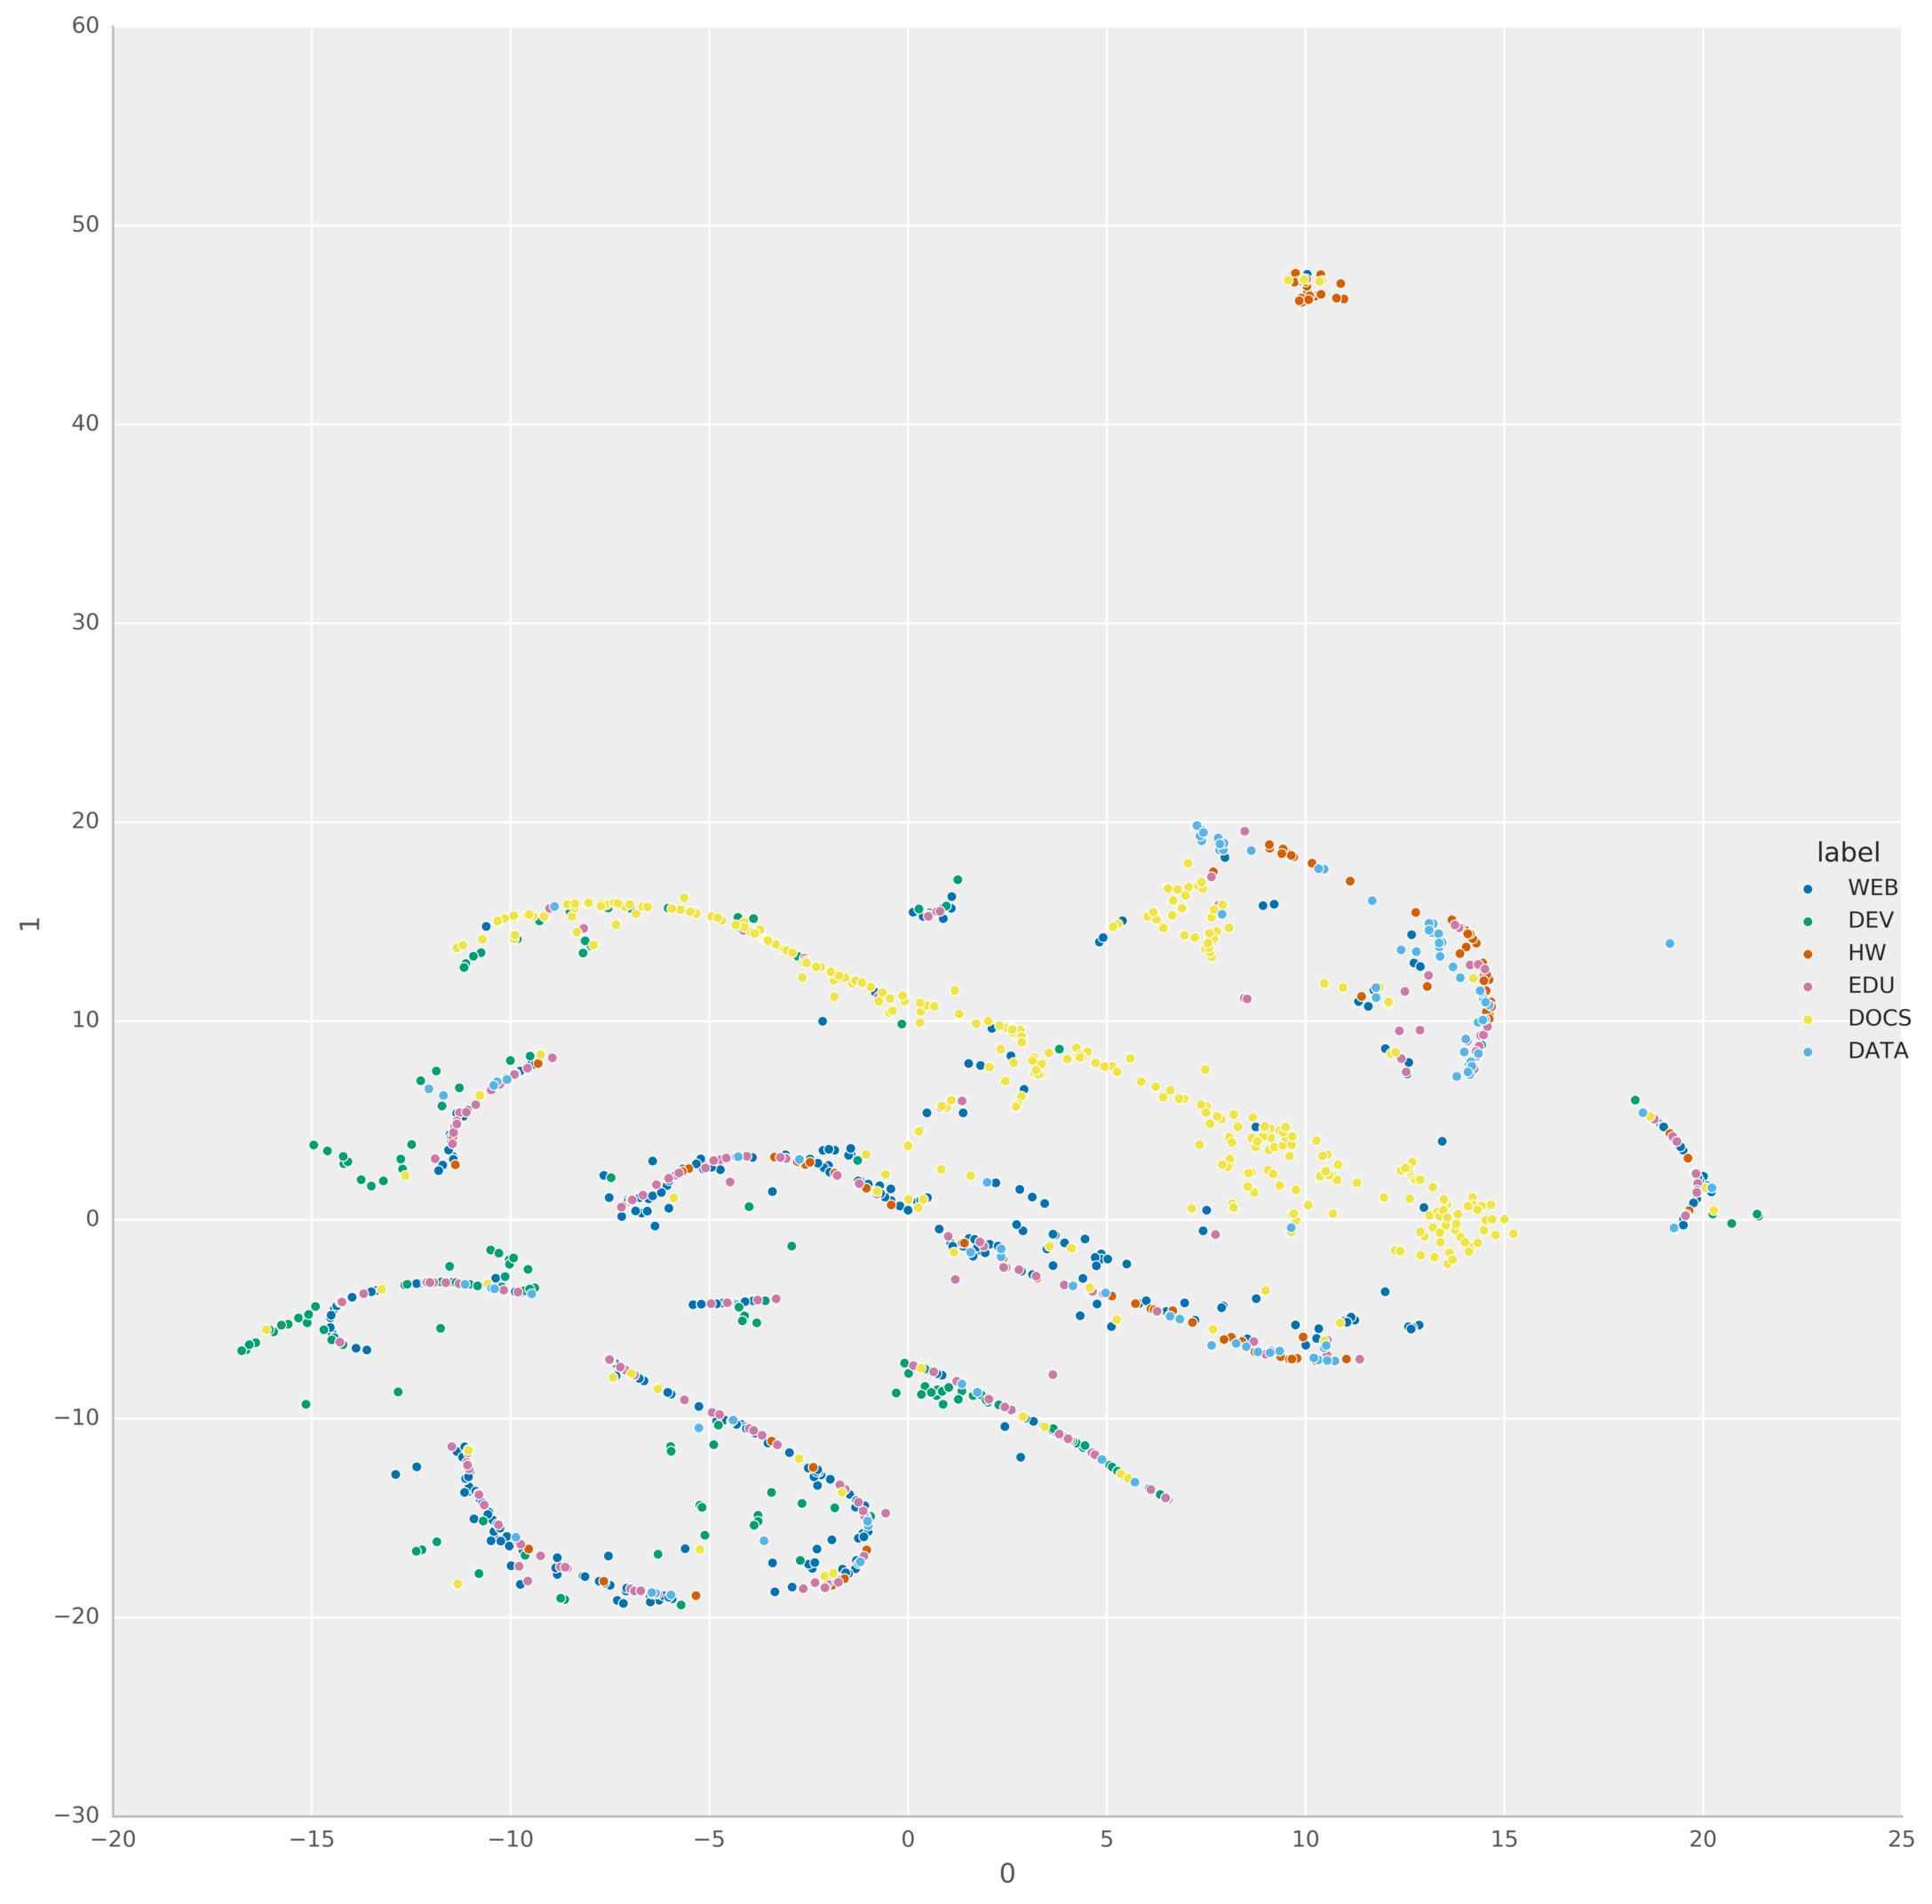
\includegraphics[width=18cm]{graphics/t-sne-training-data.png}
	\caption{Distribution of the labeled data entries using t-SNE}
	\label{t-sne-training-data}
\end{figure}


\begin{figure}
	\centering
		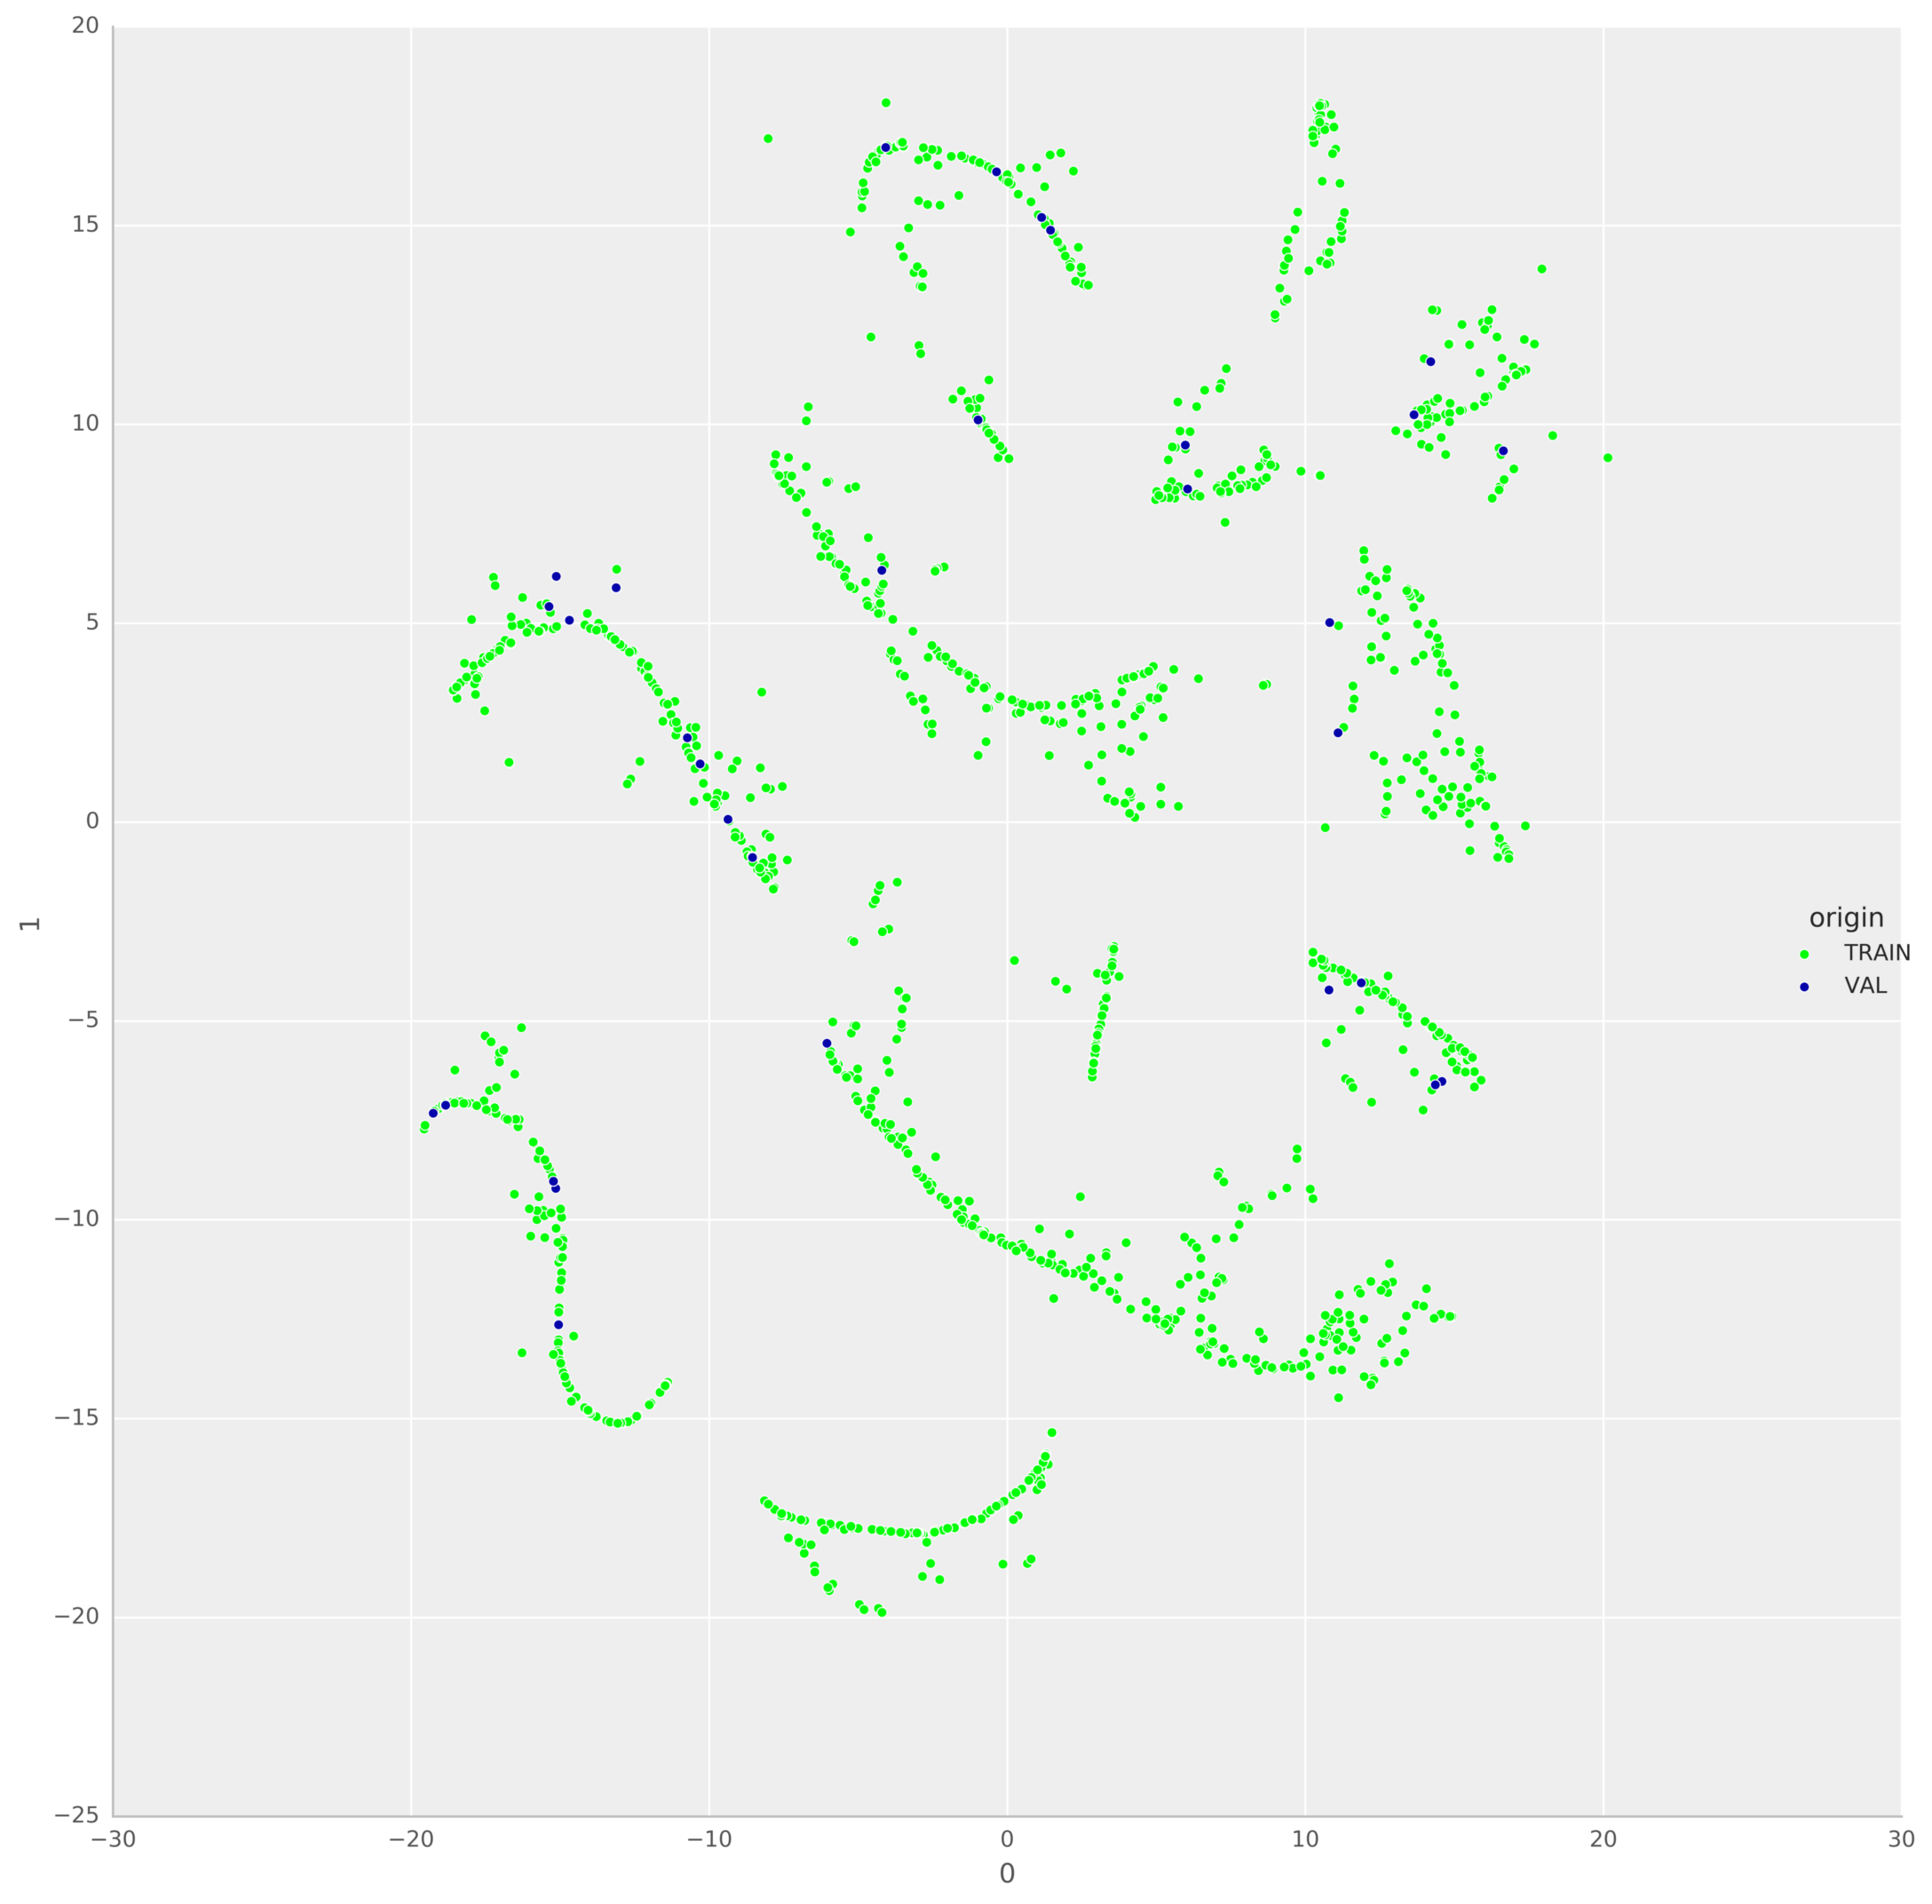
\includegraphics[width=18cm]{graphics/t-sne-validation-data.png}
	\caption{Distribution of the validation data entries using t-SNE}
	\label{t-sne-validation-data}
\end{figure}


\begin{figure}
	\centering
		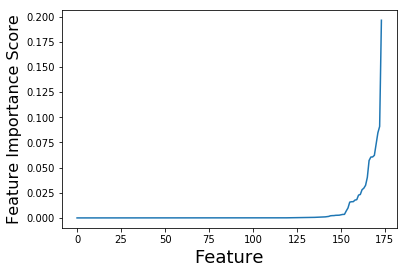
\includegraphics[width=12cm]{graphics/feature_importance_numeric.png}
	\caption{Feature Importance Scores for Numeric Features}
	\label{feature_importance_numeric_graphic}
\end{figure}

\begin{table}[h]
\centering
\caption{Top 20 Most Important Numeric Features}
\label{feature_importance_numeric}
\begin{tabular}{|l|l|l|l|}
 \hline
Feature Names & Scores & Feature Names & Scores \\ \hline
isOwnerHomepage  &   0.1793 & hasHomepage & 0.1297 \\ \hline
stargazers  &   0.0726 & mentionableUsers & 0.0642 \\ \hline
size  &   0.0581 & watchers & 0.0561 \\ \hline
commitsCount  &   0.0492 & closed\_issues & 0.0415 \\ \hline
merged\_pull\_requests  &   0.0389 & open\_issues & 0.0379 \\ \hline
forks  &   0.0376 & closed\_pull\_requests & 0.0368 \\ \hline
tagsCount  &   0.0245 & branchesCount & 0.0239 \\ \hline
hasTravisConfig  &   0.0235 & open\_pull\_requests & 0.0223 \\ \hline
releasesCount  &   0.0214 & hasLicense & 0.0148 \\ \hline
hasCiConfig  &   0.0124 & LANGUAGE\_Python & 0.0090 \\ \hline
\end{tabular}
\end{table}


\begin{table}[]
\centering
\caption{Classifier on file names - DATA category}
\label{file-names-data}
\begin{tabular}{|l|l|l|l|l|}
 \hline
   & \multicolumn{2}{l}{Positive words} & \multicolumn{2}{l}
{Negative words} \\ \hline
1 & 3.2251  &              json  &  -1.5670  &           packag \\  \hline
2 & 1.1139  &           makefil  &  -1.5648  &             test \\  \hline
3 & 0.9449  &                sh  &  -1.5623  &             main \\  \hline
4 & 0.6635  &               xml  &  -1.4399  &           config \\  \hline
5 & 0.6452  &                py  &  -1.1262  &              png \\  \hline
6 & 0.4514  &             readm  &  -1.0827  &              yml \\  \hline
7 & 0.3790  &            licens  &  -0.9016  &        contribut \\  \hline
8 & 0.3784  &             index  &  -0.7405  &              jpg \\  \hline
9 & 0.3127  &               txt  &  -0.4513  &              css \\  \hline
10 & 0.1726  &          gitignor  &  -0.2326  &            travi \\  \hline
11 & 0.0919  &               pdf  &  -0.2206  &             util \\  \hline
12 & 0.0861  &                md  &  -0.1236  &             html \\  \hline
13& &  &  -0.0684  &              svg \\  \hline
14& &  &  -0.0304  &               js \\  \hline
\end{tabular}
\end{table}
\begin{table}[]
\centering
\caption{Classifier on file names - DEV category}
\label{file-names-dev}
\begin{tabular}{|l|l|l|l|l|}
 \hline
   & \multicolumn{2}{l}{Positive words} & \multicolumn{2}{l}
{Negative words} \\ \hline
1 & 3.4637  &              util  &  -1.9203  &              pdf \\  \hline
2 & 2.3105  &            packag  &  -1.0563  &            travi \\  \hline
3 & 1.8472  &               yml  &  -0.9946  &              css \\  \hline
4 & 1.7875  &              test  &  -0.5838  &            readm \\  \hline
5 & 1.4706  &                sh  &  -0.5619  &               md \\  \hline
6 & 1.4247  &                js  &  -0.3192  &         gitignor \\  \hline
7 & 1.3238  &              html & & \\  \hline
8 & 1.2926  &           makefil & & \\  \hline
9 & 0.9907  &            config & & \\  \hline
10 & 0.9156  &              main & & \\  \hline
11 & 0.7826  &               png & & \\  \hline
12 & 0.7679  &            licens & & \\  \hline
13 & 0.7235  &             index & & \\  \hline
14 & 0.7082  &               xml & & \\  \hline
15 & 0.5805  &               txt & & \\  \hline
16 & 0.4977  &                py & & \\  \hline
17 & 0.3078  &         contribut & & \\  \hline
18 & 0.2526  &              json & & \\  \hline
19 & 0.1224  &               jpg & & \\  \hline
20 & 0.0541  &               svg & & \\  \hline
\end{tabular}
\end{table}
\begin{table}[]
\centering
\caption{Classifier on file names - DOCS category}
\label{file-names-docs}
\begin{tabular}{|l|l|l|l|l|}
 \hline
   & \multicolumn{2}{l}{Positive words} & \multicolumn{2}{l}
{Negative words} \\ \hline
1 & 4.5622  &         contribut  &  -1.0314  &           config \\  \hline
2 & 2.8728  &             travi  &  -1.0044  &             html \\  \hline
3 & 2.0420  &               yml  &  -0.7121  &              xml \\  \hline
4 & 1.7639  &            licens  &  -0.6340  &             json \\  \hline
5 & 1.7214  &                md  &  -0.5722  &          makefil \\  \hline
6 & 1.2027  &            packag  &  -0.5702  &             main \\  \hline
7 & 1.1108  &               svg  &  -0.5697  &             test \\  \hline
8 & 0.6831  &               png  &  -0.5455  &               sh \\  \hline
9 & 0.6714  &             index  &  -0.4359  &               py \\  \hline
10 & 0.3497  &             readm  &  -0.4040  &              txt \\  \hline
11 & 0.2890  &               css  &  -0.3430  &               js \\  \hline
12 & 0.2780  &               jpg  &  -0.2187  &              pdf \\  \hline
13& &  &  -0.1440  &             util \\  \hline
14& &  &  -0.0722  &         gitignor \\  \hline
\end{tabular}
\end{table}
\begin{table}[]
\centering
\caption{Classifier on file names - EDU category}
\label{file-names-edu}
\begin{tabular}{|l|l|l|l|l|}
 \hline
   & \multicolumn{2}{l}{Positive words} & \multicolumn{2}{l}
{Negative words} \\ \hline
1 & 1.7966  &               pdf  &  -1.9717  &        contribut \\  \hline
2 & 1.5195  &              html  &  -1.2080  &              yml \\  \hline
3 & 1.3308  &               jpg  &  -1.1482  &             util \\  \hline
4 & 1.0053  &               svg  &  -0.8443  &             json \\  \hline
5 & 0.9685  &               png  &  -0.2571  &           packag \\  \hline
6 & 0.8496  &          gitignor & & \\  \hline
7 & 0.6726  &                py & & \\  \hline
8 & 0.6248  &           makefil & & \\  \hline
9 & 0.5158  &            licens & & \\  \hline
10 & 0.4517  &               css & & \\  \hline
11 & 0.4501  &               txt & & \\  \hline
12 & 0.4491  &               xml & & \\  \hline
13 & 0.4232  &                sh & & \\  \hline
14 & 0.3983  &                js & & \\  \hline
15 & 0.3342  &              main & & \\  \hline
16 & 0.3019  &              test & & \\  \hline
17 & 0.2778  &             readm & & \\  \hline
18 & 0.1407  &                md & & \\  \hline
19 & 0.1085  &             travi & & \\  \hline
20 & 0.1042  &            config & & \\  \hline
\end{tabular}
\end{table}
\begin{table}[]
\centering
\caption{Classifier on file names - HW category}
\label{file-names-hw}
\begin{tabular}{|l|l|l|l|l|}
 \hline
   & \multicolumn{2}{l}{Positive words} & \multicolumn{2}{l}
{Negative words} \\ \hline
1 & 2.0428  &               css  &  -1.5755  &        contribut \\  \hline
2 & 1.7615  &              main  &  -1.3501  &           licens \\  \hline
3 & 1.5388  &            config  &  -1.0360  &              yml \\  \hline
4 & 1.2715  &          gitignor  &  -0.8501  &            travi \\  \hline
5 & 0.9140  &               txt  &  -0.8123  &              svg \\  \hline
6 & 0.7449  &             readm  &  -0.8035  &             util \\  \hline
7 & 0.5342  &                py  &  -0.5982  &           packag \\  \hline
8 & 0.5257  &              test  &  -0.4826  &             json \\  \hline
9 & 0.4687  &               xml  &  -0.3102  &          makefil \\  \hline
10 & 0.4144  &             index  &  -0.2012  &               sh \\  \hline
11 & 0.3984  &               pdf  &  -0.1943  &             html \\  \hline
12 & 0.3699  &                js  &  -0.1773  &              png \\  \hline
13 & 0.3128  &                md & & \\  \hline
14 & 0.2245  &               jpg & & \\  \hline
\end{tabular}
\end{table}
\begin{table}[]
\centering
\caption{Classifier on file names - WEB category}
\label{file-names-web}
\begin{tabular}{|l|l|l|l|l|}
 \hline
   & \multicolumn{2}{l}{Positive words} & \multicolumn{2}{l}
{Negative words} \\ \hline
1& &  &  -2.4446  &               md \\  \hline
2& &  &  -2.0628  &            readm \\  \hline
3& &  &  -1.9461  &               js \\  \hline
4& &  &  -1.9392  &              txt \\  \hline
5& &  &  -1.9117  &             html \\  \hline
6& &  &  -1.9110  &              png \\  \hline
7& &  &  -1.8890  &             json \\  \hline
8& &  &  -1.8842  &               py \\  \hline
9& &  &  -1.8702  &              xml \\  \hline
10& &  &  -1.8512  &              pdf \\  \hline
11& &  &  -1.8435  &         gitignor \\  \hline
12& &  &  -1.7930  &            travi \\  \hline
13& &  &  -1.7274  &             test \\  \hline
14& &  &  -1.7246  &           config \\  \hline
15& &  &  -1.7224  &              jpg \\  \hline
16& &  &  -1.7115  &             main \\  \hline
17& &  &  -1.7010  &              css \\  \hline
18& &  &  -1.6888  &          makefil \\  \hline
19& &  &  -1.6295  &           licens \\  \hline
20& &  &  -1.6165  &            index \\  \hline
\end{tabular}
\end{table}
